\renewcommand*{\arraystretch}{1.1}

\subsection*{BI / read / 22}
\label{section:bi-read-22}

% change \emph{} to use sans-serif font
\let\oldemph\emph
\renewcommand{\emph}[1]{{\footnotesize \sf #1}}

\renewcommand{\currentQueryCard}{22}
\marginpar{
	\raggedleft
	\vspace{0.22ex}

	\queryRefCard{bi-read-01}{BI}{1}\\
	\queryRefCard{bi-read-02}{BI}{2}\\
	\queryRefCard{bi-read-03}{BI}{3}\\
	\queryRefCard{bi-read-04}{BI}{4}\\
	\queryRefCard{bi-read-05}{BI}{5}\\
	\queryRefCard{bi-read-06}{BI}{6}\\
	\queryRefCard{bi-read-07}{BI}{7}\\
	\queryRefCard{bi-read-08}{BI}{8}\\
	\queryRefCard{bi-read-09}{BI}{9}\\
	\queryRefCard{bi-read-10}{BI}{10}\\
	\queryRefCard{bi-read-11}{BI}{11}\\
	\queryRefCard{bi-read-12}{BI}{12}\\
	\queryRefCard{bi-read-13}{BI}{13}\\
	\queryRefCard{bi-read-14}{BI}{14}\\
	\queryRefCard{bi-read-15}{BI}{15}\\
	\queryRefCard{bi-read-16}{BI}{16}\\
	\queryRefCard{bi-read-17}{BI}{17}\\
	\queryRefCard{bi-read-18}{BI}{18}\\
	\queryRefCard{bi-read-19}{BI}{19}\\
	\queryRefCard{bi-read-20}{BI}{20}\\
	\queryRefCard{bi-read-21}{BI}{21}\\
	\queryRefCard{bi-read-22}{BI}{22}\\
	\queryRefCard{bi-read-23}{BI}{23}\\
	\queryRefCard{bi-read-24}{BI}{24}\\
	\queryRefCard{bi-read-25}{BI}{25}\\
}



\noindent\begin{tabularx}{\queryCardWidth}{|>{\queryPropertyCell}p{\queryPropertyCellWidth}|X|}
	\hline
	query & BI / read / 22 \\ \hline
%
	title & International dialog \\ \hline
%
	pattern & \multicolumn{1}{c|}{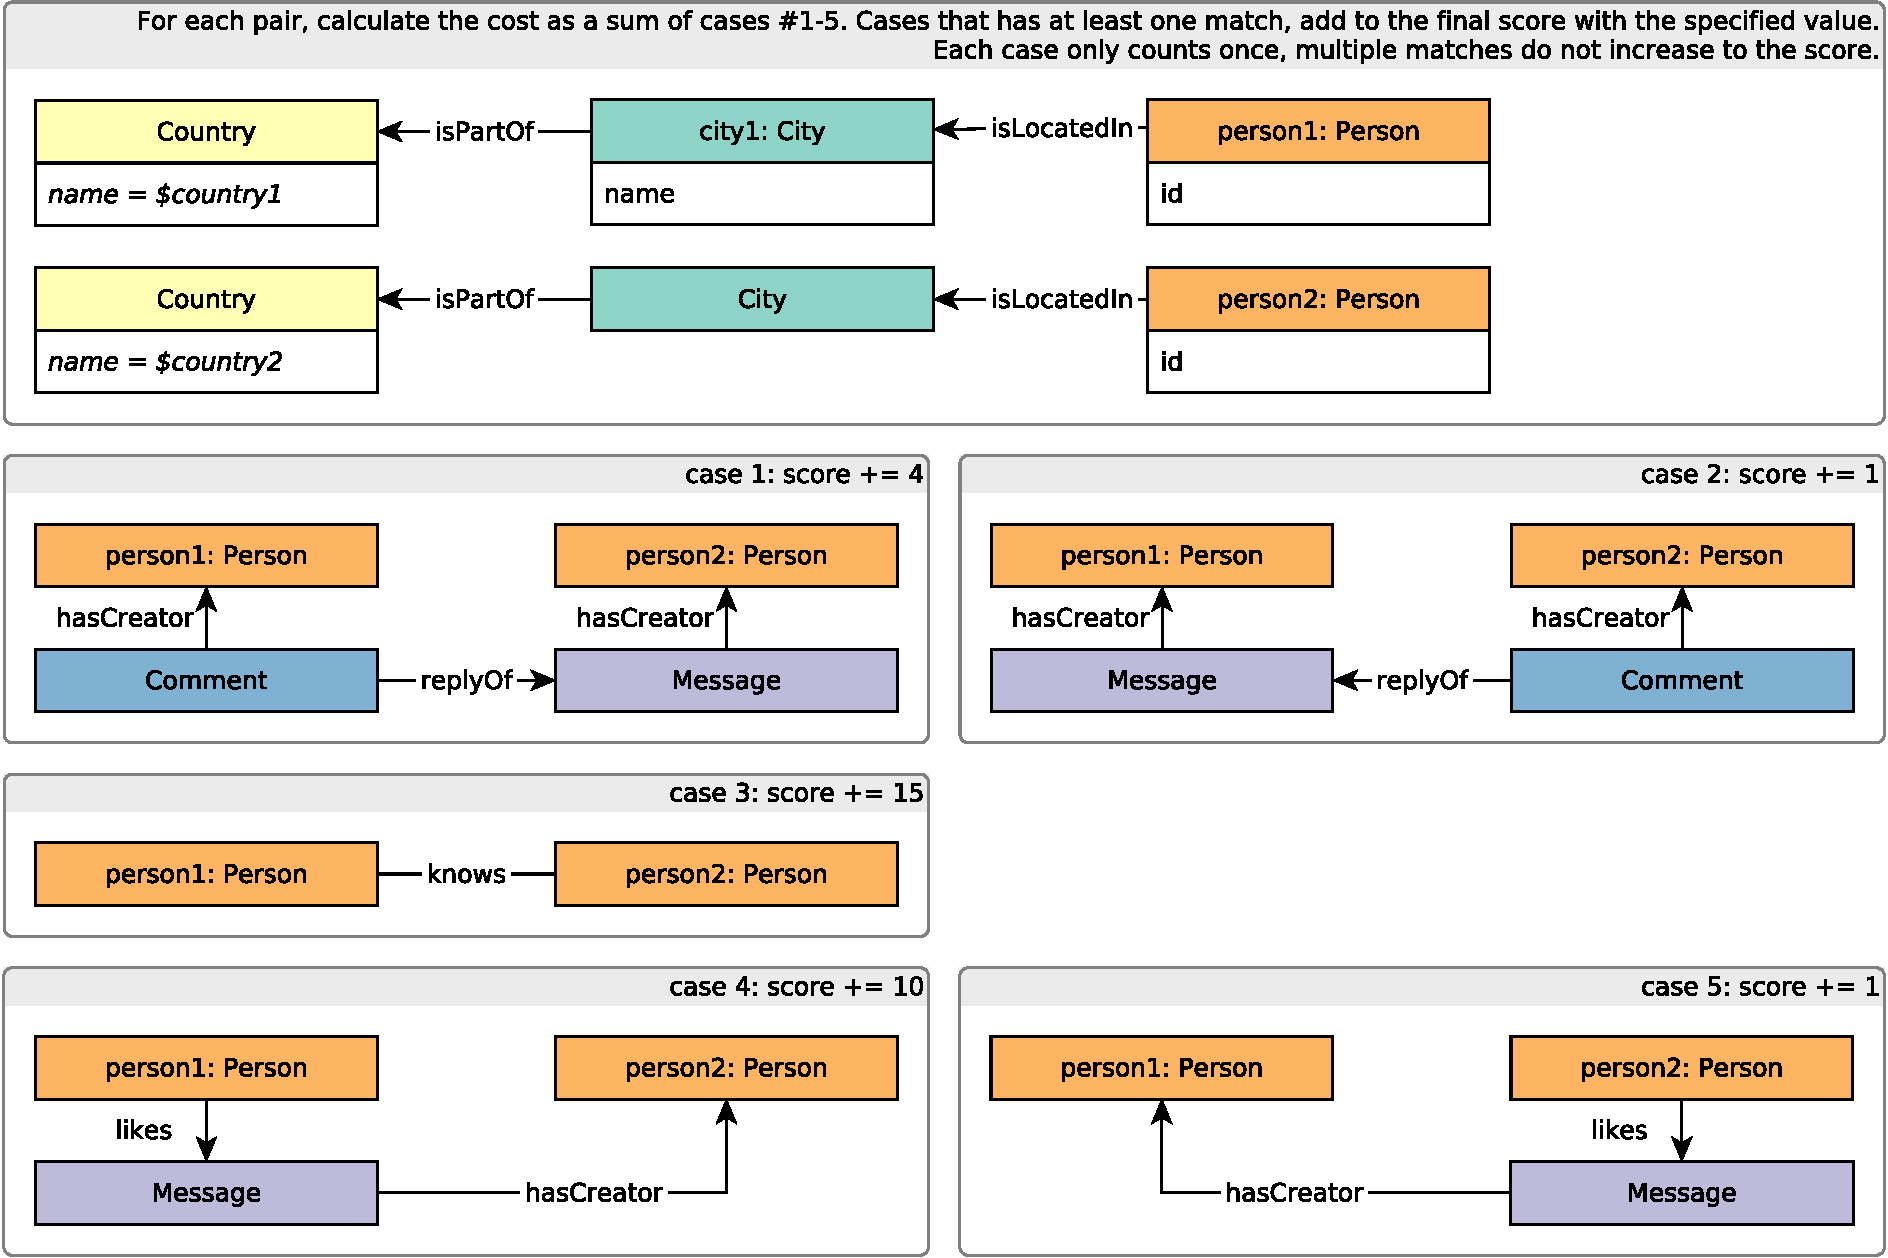
\includegraphics[scale=\patternscale,margin=0cm .2cm]{patterns/bi-read-22}} \\ \hline
%
	desc. & Consider all pairs of people \texttt{(person1,\ person2)} such that one
is located in a \emph{City} of \emph{Country} \texttt{country1} and the
other is located in a \emph{City} of \emph{Country} \texttt{country2}.
For each \emph{City} of \emph{Country} \texttt{country1}, return the
highest scoring pair. The score of a pair is defined as the sum of the
subscores awarded for the following kinds of interaction. The initial
value is \texttt{score\ =\ 0}.

\begin{enumerate}
\def\labelenumi{\arabic{enumi}.}
\tightlist
\item
  \texttt{person1} has created a reply \emph{Comment} to at least one
  \emph{Message} by \texttt{person2}: \texttt{score\ +=\ 4}
\item
  \texttt{person1} has created at least one \emph{Message} that
  \texttt{person2} has created a reply \emph{Comment} to:
  \texttt{score\ +=\ 1}
\item
  \texttt{person1} and \texttt{person2} \emph{know} each other:
  \texttt{score\ +=\ 15}
\item
  \texttt{person1} liked at least one \emph{Message} by
  \texttt{person2}: \texttt{score\ +=\ 10}
\item
  \texttt{person1} has created at least one \emph{Message} that was
  liked by \texttt{person2}: \texttt{score\ +=\ 1}
\end{enumerate}

Consequently, the maximum score a pair can obtain is:
\texttt{4\ +\ 1\ +\ 15\ +\ 10\ +\ 1\ =\ 31}.

To break ties, order by (1) \texttt{person1.id} ascending and (2)
\texttt{person2.id} ascending.
 \\ \hline
%
	
		params &
		\innerCardVSpace{\begin{tabularx}{\attributeCardWidth}{|>{\paramNumberCell}c|>{\varNameCell}M|>{\typeCell}m{\typeWidth}|Y|} \hline
		$\mathsf{1}$ & country1
 & String
 &  \\ \hline
		$\mathsf{2}$ & country2
 & String
 &  \\ \hline
		\end{tabularx}}\innerCardVSpace \\ \hline
	
%
	
		result &
		\innerCardVSpace{\begin{tabularx}{\attributeCardWidth}{|>{\resultNumberCell}c|>{\varNameCell}M|>{\typeCell}m{\typeWidth}|>{\resultOriginCell}c|Y|} \hline
		$\mathsf{1}$ & person1.id & 64-bit Integer & R &
				 \\ \hline
		$\mathsf{2}$ & person2.id & 64-bit Integer & R &
				 \\ \hline
		$\mathsf{3}$ & city1.name & String & R &
				 \\ \hline
		$\mathsf{4}$ & score & 32-bit Integer & C &
				 \\ \hline
		\end{tabularx}}\innerCardVSpace \\ \hline
	
%
	
		sort		&
		\innerCardVSpace{\begin{tabularx}{\attributeCardWidth}{|>{\sortNumberCell}c|>{\varNameCell}M|>{\directionCell}c|Y|} \hline
		$\mathsf{1}$ & score
 & $\desc
$ &  \\ \hline
		$\mathsf{2}$ & person1.id
 & $\asc
$ &  \\ \hline
		$\mathsf{3}$ & person2.id
 & $\asc
$ &  \\ \hline
		\end{tabularx}}\innerCardVSpace \\ \hline
	%
	%
	CPs &
	\multicolumn{1}{>{\raggedright}l|}{
		\chokePoint{1.3}, 
		\chokePoint{1.4}, 
		\chokePoint{2.1}, 
		\chokePoint{3.1}, 
		\chokePoint{3.3}, 
		\chokePoint{5.1}, 
		\chokePoint{5.2}, 
		\chokePoint{5.3}, 
		\chokePoint{8.3}, 
		\chokePoint{8.4}
		} \\ \hline
	%
	%
\end{tabularx}
\queryCardVSpace

% change \emph back to the old one
\let\emph\oldemph